\begin{spacing}{.5}
  \chapter*{Abstract}
\end{spacing}
The Doka company offers software packages to their customers. Here is the administration
still very much in need of improvement. The process of adding new software packages,
works as follows: creating new packages, editing and deleting
takes place directly via the database, which means that there is no administration program
to date. Since everything runs through the database, it becomes clean
work prevented. That's why we were commissioned by the Doka company to create a
Database Management System based on the JavaScript library React. 
Before some terms need to be explained:
\\
\\
It should be possible to manage the following tables that have these properties: 
\\
\\
- InstallablePackage is the main table, consists of several Installables and
can have a description (InstallablaPackagesDesciptions) in multiple languages. 
\\
- An Installable has an InstallableSyncTemplate and can have an InstallableExecutablePaths.
\\
\\
The program should have the following functions:
\\
\\
- Viewing, installing, adding, editing and deleting so-called
\\
Installables / InstallablePackages / InstallableSyncTemplates / InstallableExecutablePaths 
- Exporting the current configuration 
\\
- Importing a JSON file,
where to see the difference of the imported file and the current configuration 
\\
- Reset the cache in the backend

\begin{figure}
  \centering
  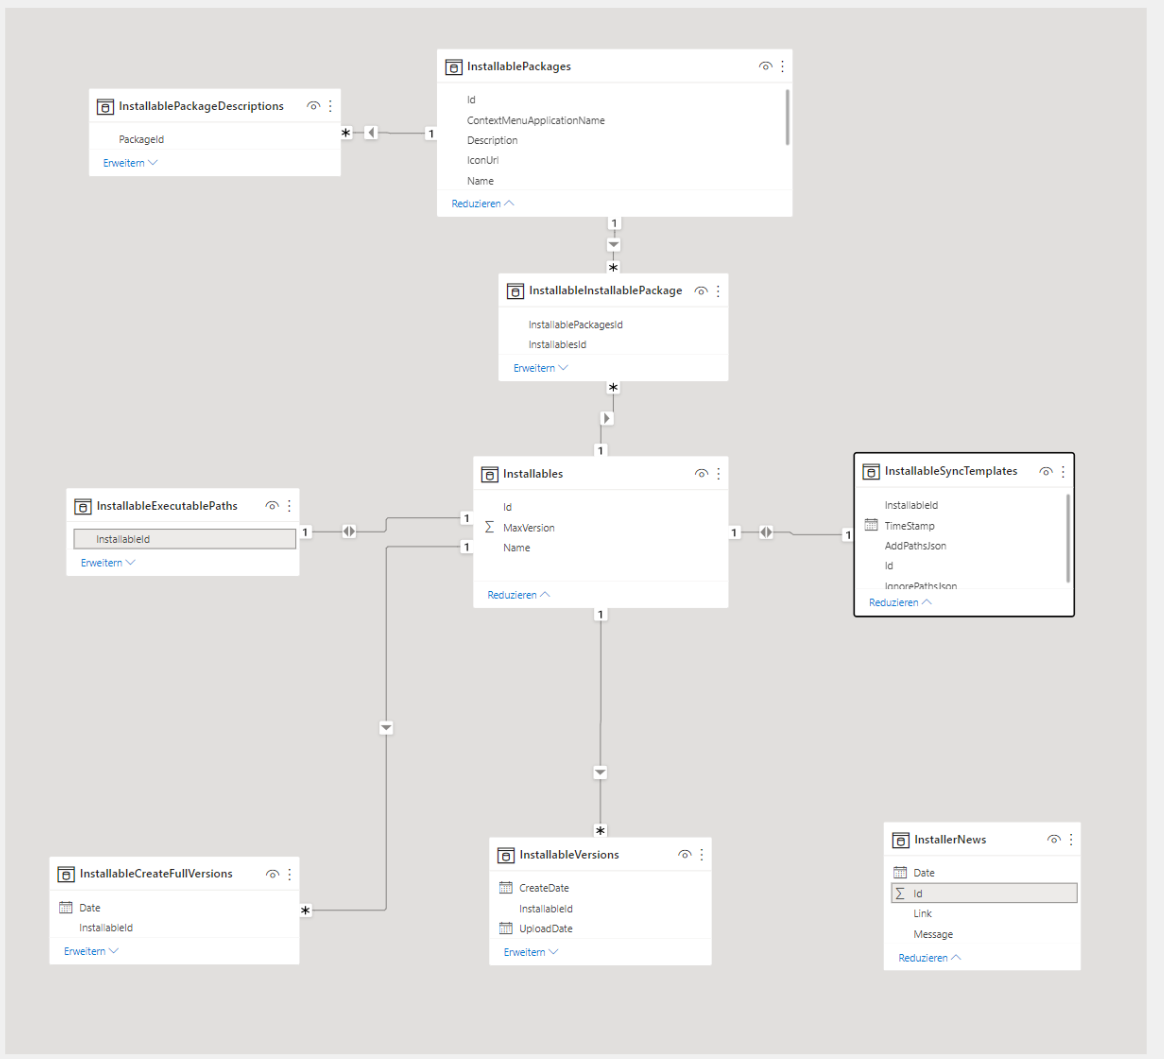
\includegraphics[width=.94\textwidth]{pics/erd.png}
  \caption{\label{fig:The-caption} ERD}
\end{figure}

\newpage
\begin{spacing}{.5}
  \chapter*{Zusammenfassung}
\end{spacing}
Die Firma Doka bietet Softwarepakete an deren Kunden an. Dabei ist das Verwalten noch sehr verbesserungswürdig.
Der Prozess des hinzufügens von neuen Softwarepaketen, läuft wiefolgt ab:
Das Erstellen von neuen Paketen, das Editieren sowie das Löschen erfolgt direkt über die Datenbank, das bedeutet, dass
es kein Verwaltungsprogramm bis dato gibt. Dadruch, dass alles über die Datenbank abläuft, wird das saubere Arbeiten
verhindert. Deshalb wurden wir von der Firma Doka dazu beauftragt, ein Verwaltungssystem basierend auf der JavaScript library
React zu programmieren. Davor müssen einige Begriffe noch erklärt werden:
\\
\\
Folgende Tabellen sollen verwaltet werden können, die diese Eigenschaften haben:
\\
\\
- InstallablePackage ist die wichtigste Tabelle, besteht aus mehreren Installables und kann Beschreibung (InstallablaPackagesDesciptions) auf mehreren Sprachen haben.
\\
- Ein Installable hat ein InstallableSyncTemplate und kann ein InstallableExecutablePaths.
\\
\\
Dabei soll das Programm folgende Funktionen haben:
\\
\\
- Das Anzeigen, Installieren, Hinzufügen, Bearbeiten und Löschen von sogenannten Installables / InstallablePackages / InstallableSyncTemplates / InstallableExecutablePaths
\\
- Das Exportieren der aktuellen Konfiguration
\\
- Importieren eines JSON Dateis, wo die Differenz der importierten Datei und der aktuellen Konfiguration zu sehen ist
\\  
- Reseten des Cache im Backend

\begin{figure}
  \centering
  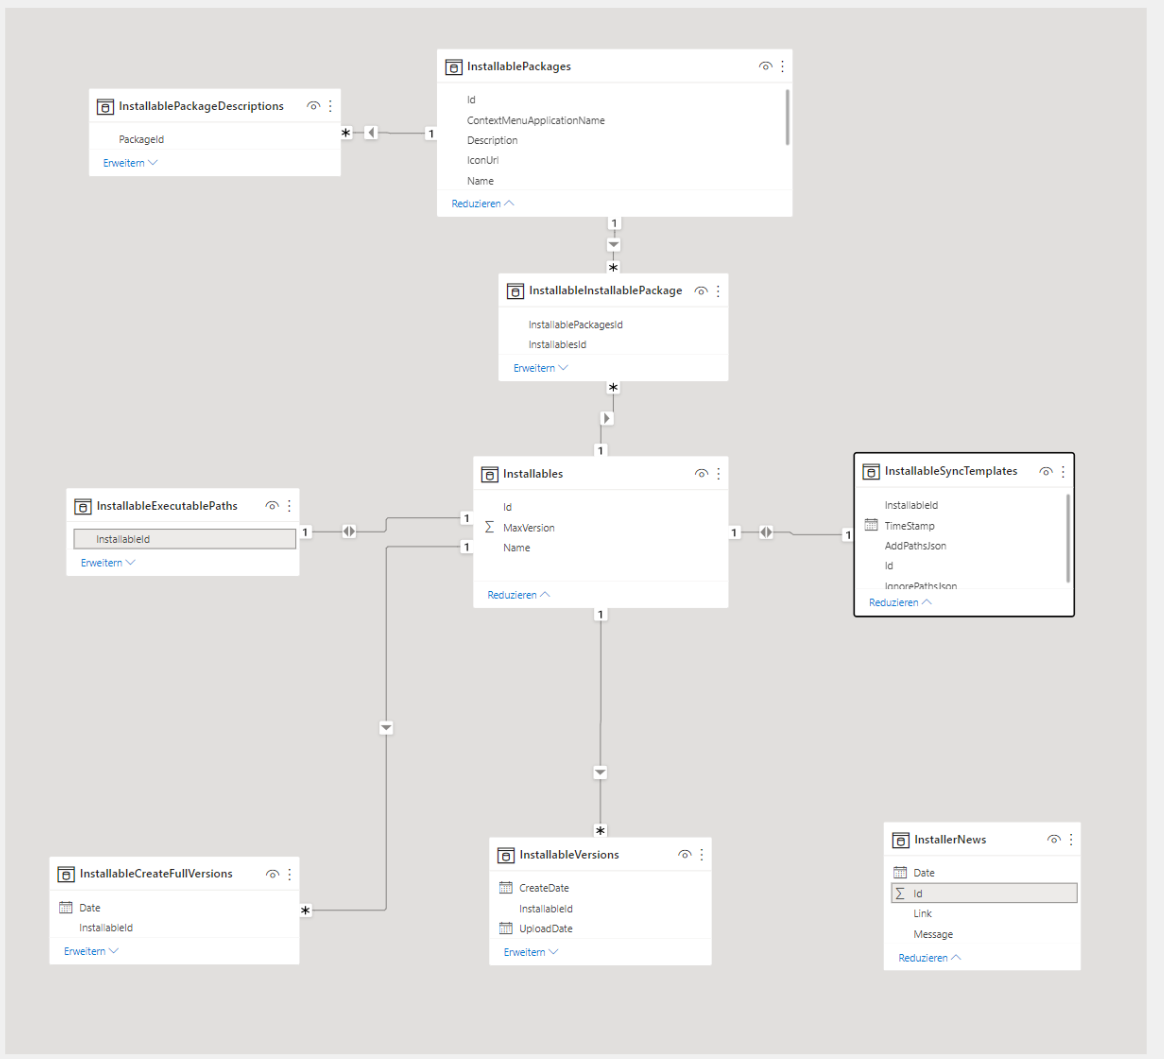
\includegraphics[width=.94\textwidth]{pics/erd.png}
  \caption{\label{fig:The-caption}ERD}
\end{figure}

%\emph{Bitte auf keinen Fall mit der Zusammenfassung verwechseln, die den Abschluss der Arbeit bildet!}